\documentclass[../../main.tex]{subfiles}
\graphicspath{{../../image/}{../../figure/}}
\begin{document}

\section{真非线性守恒律系统的前沿追踪}\label{section:ch14-真非线性系统的前沿追踪}

考虑典范形式的守恒律系统
\begin{align}
\partial_t U+\partial_x F(U)=0,
\label{align:ch14-system}
\end{align}
它是严格双曲的\eqref{align:ch07-严格双曲不等式}，且每个特征族要么真非线性\eqref{align:ch07-真正非线性条件}，要么线性退化\eqref{align:ch07-线性退化条件}。本节目的是引入一种前沿追踪算法，它求解初值问题\eqref{align:ch13-ivp}（初值 $U_0$ 总变差很小），并特别给出存在性定理\eqref{align:ch13-ivp}的一个替代证明。



该算法的工具将是特殊 Riemann 解算器，用于把跳跃间断分解为以跳跃间断与常状态组成的中心波扇，逼近 Riemann 问题的可容许解。在实现算法时，先把初值用阶梯函数逼近，其跳跃间断继而分解为波扇。由跳跃间断碰撞诱发的相互作用按其发生顺序同样分解为类似波扇。只需考虑一般情形，即至多两个跳跃间断同时碰撞。预期此种构造将在分段常值函数类中产生初值问题的近似解。

首要议题是如何设计合适的 Riemann 解算器。\cref{section:ch14-标量守恒律的前沿追踪}中标量守恒律的经验提示：应通过常状态、可容许激波与小强度不可容许稀疏激波的组合来合成中心波扇。

在可容许 $i$-激波中，右端状态 $U_+$ 位于通过左端状态 $U_-$ 的第 $i$ 激波曲线上，即按\cref{section:ch09-用波曲线求解riemann问题}的记号 $U_+=\Phi_i(\tau;U_-)$；当第 $i$ 特征族真非线性时 $\tau<0$（压缩激波），当第 $i$ 特征族线性退化时 $\tau\lessgtr0$（接触间断）。振幅为 $\tau$，强度以 $|\tau|$ 度量，速度 $s$ 由 Rankine--Hugoniot 跳跃条件\eqref{align:ch08-rh}给定。



与其用真正的稀疏激波，不如采用``稀疏前沿''，即连接位于稀疏波曲线上并以特征速度传播的状态的跳跃间断更为方便。因而，$i$-稀疏前沿（仅当第 $i$ 特征族真非线性时才可能出现）中右端状态 $U_+$ 位于通过左端状态 $U_-$ 的第 $i$ 稀疏波曲线上，即 $U_+=\Phi_i(\tau;U_-)$，$\tau>0$。振幅与强度均以 $\tau$ 度量，速度取为 $\lambda_i(U_+)$。显然，这些前沿不仅违反熵可容性准则，甚至也违反 Rankine--Hugoniot 跳跃条件，尽管当其强度很小时仅略有违反。

中心稀疏波可由常状态与强度不超过某预定值 $\delta>0$ 的稀疏前沿组成的复合波逼近。取某 $i$-稀疏波，为确定起见中心位于原点，左端连接状态 $U_-$、右端连接状态 $U_+$。于是 $U_+$ 位于通过 $U_-$ 的 $i$-稀疏曲线上，即 $U_+=\Phi_i(\tau;U_-)$，某 $\tau>0$。令 $\nu$ 为大于 $\tau/\delta$ 的最小整数。置 $U^0=U_-$、$U^\nu=U_+$，定义 $U^\mu=\Phi_i(\mu\delta;U_-)$，$\mu=1,\cdots,\nu-1$，并用扇区 $\lambda_i(U_-)<\frac{x}{t}<\lambda_i(U_+)$ 内的波扇
\begin{align}
U(x,t)=U^\mu,\qquad \lambda_i(U^{\mu-1})<\frac{x}{t}<\lambda_i(U^\mu),\qquad \mu=1,\cdots,\nu
\label{align:ch14-rarefaction-fan}
\end{align}
来逼近该稀疏波。

由此自然引出近似 Riemann 解算器：它按如下手续把左端状态 $U_l$ 与右端状态 $U_r$ 之间的跳跃间断分解为由常状态、可容许激波与稀疏前沿组成的波扇。出发点是 Riemann 问题的可容许解，它由 $n+1$ 个常状态 $U_l=U_0,U_1,\cdots,U_n=U_r$ 组成，其中 $U_{i-1}$ 与 $U_i$ 由可容许 $i$-激波或 $i$-稀疏波连接。过渡到近似时，保留常状态的定义域与取值（从而保留所有激波），而按上述在其扇区内用同族常状态与稀疏前沿的扇替换任一稀疏波，前沿强度不超过 $\delta$（见\cref{figure:ch14-近似riemann解算器}）。

\begin{figure}[ht]
\centering
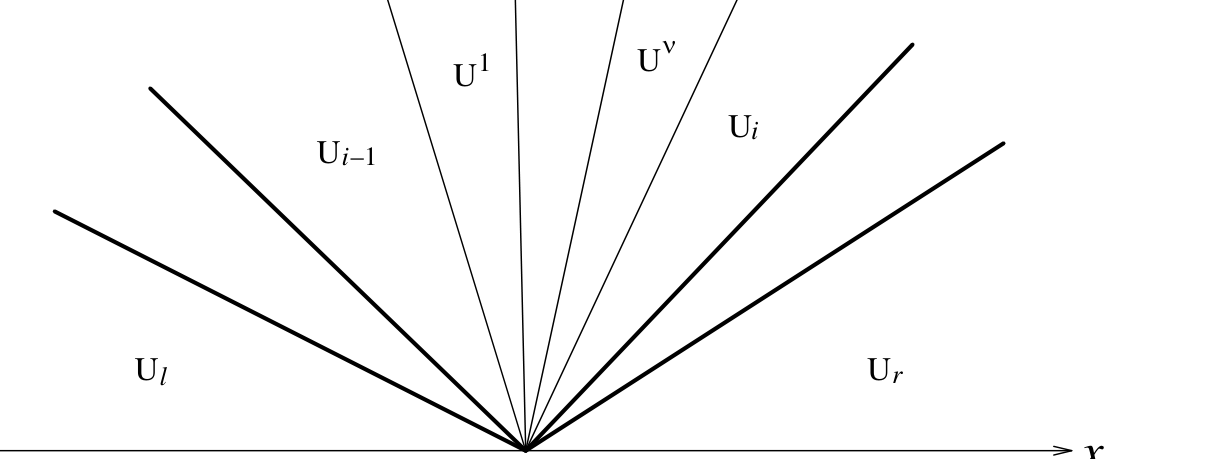
\includegraphics[width=0.8\textwidth]{ch14-fig02-01.png}
\caption{近似 Riemann 解算器产生的波扇}\label{figure:ch14-近似riemann解算器}
\end{figure}

我们先前在标量情形的成功可能使人期望：一种前沿追踪算法（其中所有激波相互作用都通过上述近似但相对精确的 Riemann 解算器求解）将产生系统的近似解，并当稀疏前沿允许强度 $\delta$ 收缩到零时收敛到初值问题的可容许解。不幸的是，此种方法一般会失败，原因如下：与标量守恒律情形相反，系统中的波相互作用倾向于增加波型的复杂性，使碰撞变得越来越频繁，算法可能在有限时间内停滞不前。作为补救，为阻止波的大量增殖，只有强度可观的激波与稀疏前沿才以相对精度追踪；其余波不完全忽略，而是以较低精度处理：把它们归并为跳跃间断，称为伪激波，以人工超声速速度传播。

伪激波可连接任意状态 $U_-$ 与 $U_+$。其强度以 $|U_+-U_-|$ 度量，指定速度取为 $\lambda_n(U)$ 的固定上界 $\lambda_{n+1}$，其中 $U$ 取遍解的值域。显然，伪激波比稀疏前沿更严重地违反 Rankine--Hugoniot 跳跃条件，因而可能严重破坏近似解，除非其总强度保持很小。

为行文方便，把 $i$-稀疏前沿与 $i$-激波（压缩或接触间断）统称为 $i$-前沿。前沿与伪激波统称为波。因而 $i$-前沿是 $i$-波，伪激波称为 $(n+1)$-波。如前几章，波的振幅用希腊字母 $\alpha,\beta,\gamma,\cdots$ 表示，相应强度为 $|\alpha|,|\beta|,|\gamma|,\cdots$。

在下述将指定的情形下，由两个波碰撞产生的跳跃间断将通过简化 Riemann 解算器求解：它允许前沿穿过相互作用点而不改变其强度，同时引入一个出射伪激波以弥合状态间的失配。可能出现如下情形。

设对 $i<j$，连接状态 $U_l$ 与 $U_m$ 的 $j$-前沿与连接状态 $U_m$ 与 $U_r$ 的 $i$-前沿碰撞；见\cref{figure:ch14-不同族前沿碰撞}。于是 $U_m=\Phi_j(\tau_l;U_l)$ 且 $U_r=\Phi_i(\tau_r;U_m)$。为实现简化 Riemann 解算器，确定状态 $U_p=\Phi_i(\tau_r;U_l)$ 与 $U_q=\Phi_j(\tau_l;U_p)$。于是出射波扇由连接 $U_l$ 与 $U_p$ 的 $i$-前沿、连接 $U_p$ 与 $U_q$ 的 $j$-前沿，以及连接 $U_q$ 与 $U_r$ 的伪激波组成。

\begin{figure}[ht]
\centering
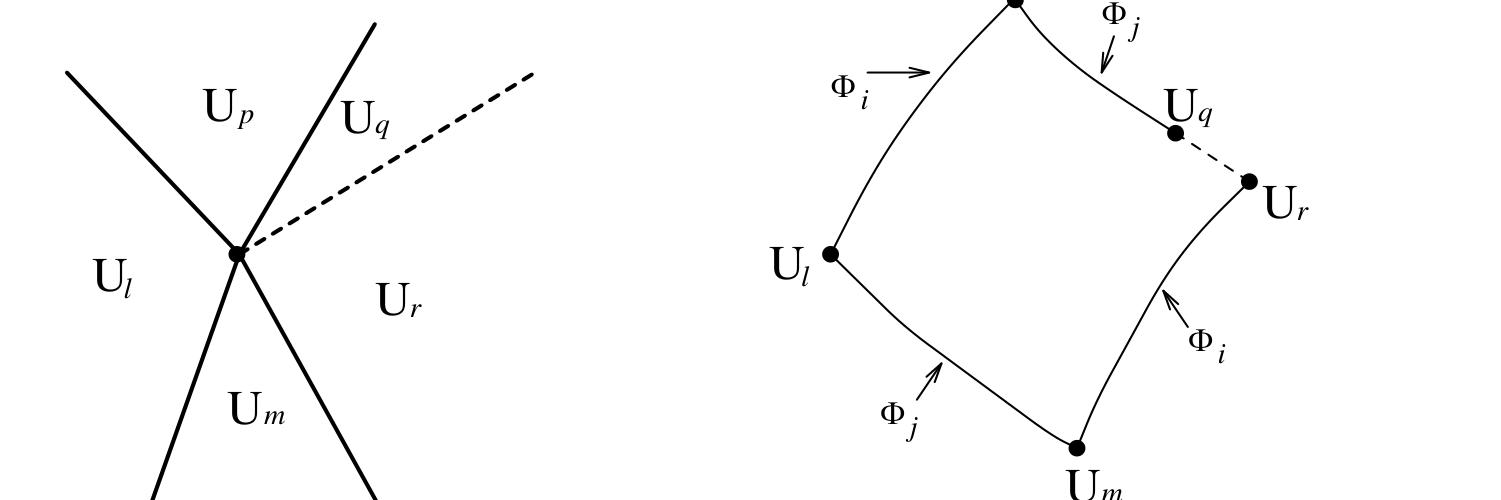
\includegraphics[width=0.9\textwidth]{ch14-fig02-02.png}
\caption{$i$-前沿与 $j$-前沿的碰撞（$i<j$）}\label{figure:ch14-不同族前沿碰撞}
\end{figure}

接着设连接状态 $U_l$ 与 $U_m$ 的 $i$-前沿与另一连接状态 $U_m$ 与 $U_r$ 的 $i$-前沿碰撞（除非至少一个前沿是压缩激波，否则此种碰撞不会发生）；见\cref{figure:ch14-同族前沿碰撞}。

于是 $U_m=\Phi_i(\tau_l;U_l)$ 且 $U_r=\Phi_i(\tau_r;U_m)$。若 $U_q=\Phi_i(\tau_l+\tau_r;U_l)$，则出射波扇由连接 $U_l$ 与 $U_q$ 的 $i$-前沿，以及连接 $U_q$ 与 $U_r$ 的伪激波组成。

\begin{figure}[ht]
\centering
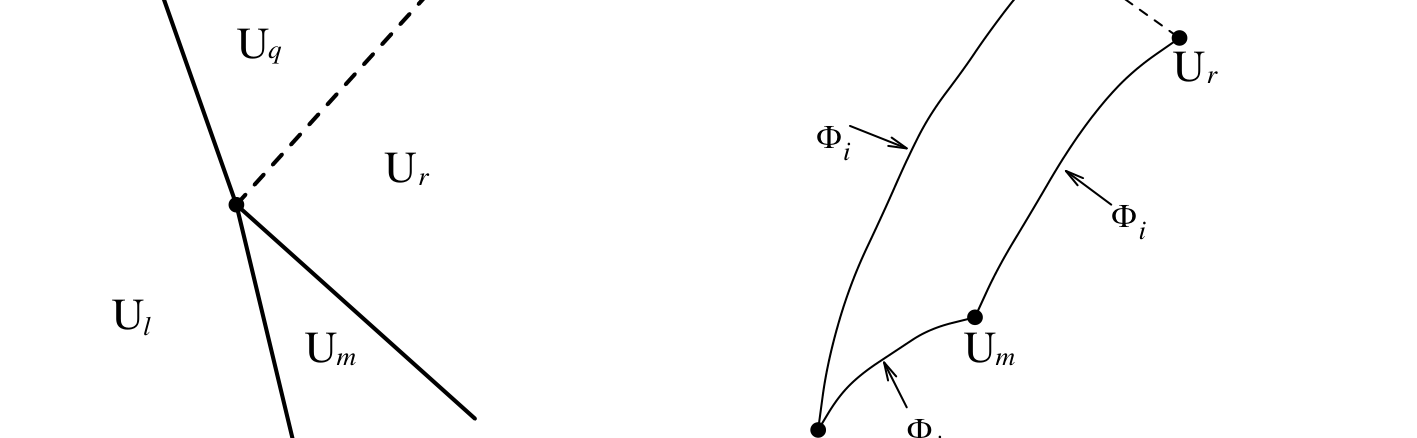
\includegraphics[width=0.9\textwidth]{ch14-fig02-03.png}
\caption{两个同族 $i$-前沿的碰撞}\label{figure:ch14-同族前沿碰撞}
\end{figure}

最后，设连接状态 $U_l$ 与 $U_m$ 的伪激波与连接状态 $U_m$ 与 $U_r$ 的 $i$-前沿碰撞；见\cref{figure:ch14-伪激波与前沿碰撞}。于是 $U_r=\Phi_i(\tau_m;U_m)$。确定 $U_q=\Phi_i(\tau_m;U_l)$。出射波扇由连接 $U_l$ 与 $U_q$ 的 $i$-前沿，以及连接 $U_q$ 与 $U_r$ 的伪激波组成。

\begin{figure}[ht]
\centering
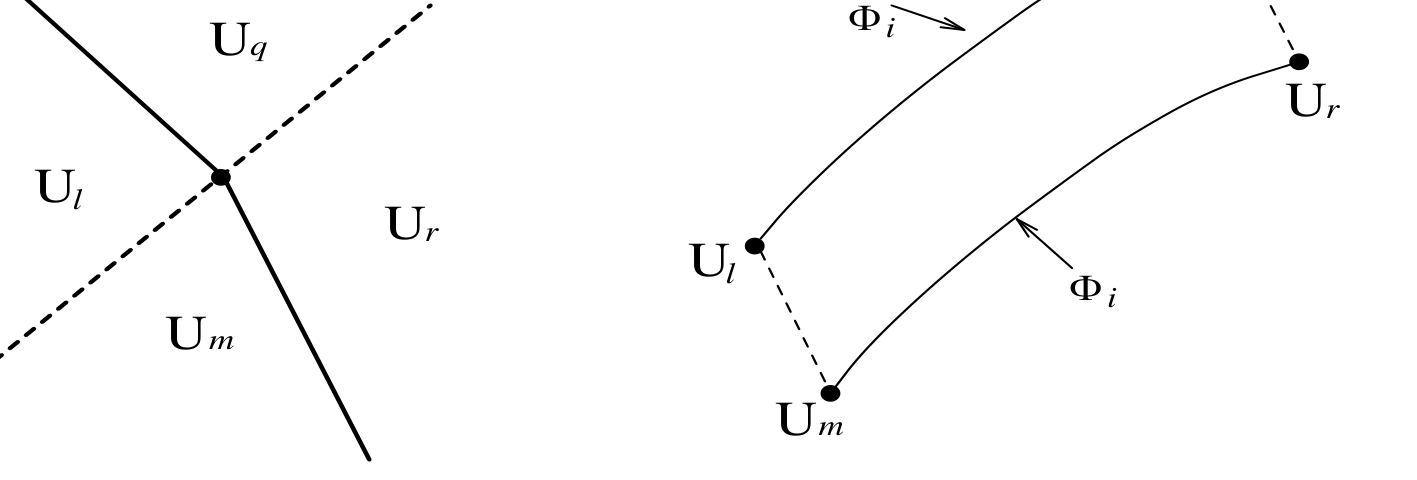
\includegraphics[width=0.9\textwidth]{ch14-fig02-04.png}
\caption{伪激波与 $i$-前沿的碰撞}\label{figure:ch14-伪激波与前沿碰撞}
\end{figure}

在实现前沿追踪算法时，一开始就固定伪激波的超声速速度 $\lambda_{n+1}$，设定稀疏前沿强度的限值 $\delta$，并指定第三个参数 $\sigma>0$，它规定跳跃间断的求解方式：
\begin{itemize}
\item 由两个前沿碰撞产生的跳跃间断，其振幅分别为 $\alpha$ 与 $\beta$，当 $|\alpha||\beta|>\sigma$ 时通过近似 Riemann 解算器求解，当 $|\alpha||\beta|\leqslant\sigma$ 时通过简化 Riemann 解算器求解。
\item 由伪激波与任一前沿碰撞产生的跳跃间断须通过简化 Riemann 解算器求解。
\item 逼近初值的阶梯函数的跳跃间断须通过近似 Riemann 解算器求解。
\end{itemize}

\end{document}
